\chapter{Churn prediction}
\label{ch:churn}

\section{Data}
\label{sec:churn_data}

The data used throughout this work is a monthly summary of customers' activity,
mobile data usage in MB, number of calls and messages, along with information
about the type of subscription, hardware, and socio-demographic information.
This amounts to a total of 73 variables. The dataset comprises one entry per
customer and per month, and a total of 5 months are present from the year 2018.
About 1.5 million entries are present per month, for a total of about 7.6
million entries in the entire dataset. The target variable, churn, is
represented as a date if the client is known to have churned, or an empty value
otherwise.

Two kinds of contracts are present in this dataset, that we will call \emph{SIM
only} and \emph{loyalty}. The first type refers to a subscription where the
customer can churn freely at any time. This differs from the second type where
the customer receives a large discount on the purchase of a mobile phone but
agrees not to churn for a certain period of time, usually 24 months. If the
customer decides nonetheless to stop his subscription before the term of the
contract, she has to pay back the remaining discount. After the data
preprocessing step (presented in section \ref{sec:data_pre}), we are left with a
total of about 5 millions entries corresponding to SIM only contracts, and about
250,000 entries corresponding to loyalty contracts. Therefore, we will mainly
focus on SIM only contracts, for its broader impact on the customer base and its
increased statistical significance. Some of the experiments will nevertheless be
conducted on both types of contracts, in order to understand the differences in
the churn dynamic.

Note that the number of entries in the loyalty dataset does not correspond to
the real number of customers having this type of contract. This is due to the
way the loyalty data entries are filtered. We focus only on customers
approaching the end of the mandatory period of the contract, since it is at
this point that the churn rate raises. Before this period of time, the churn is
almost non-existent, due to the remaining discount to be paid back by the
customer. We consider a time frame of 2 months, explaining the low number of
data entries under consideration.

Due to commercial reasons, a non-disclosure agreement prevents us from
communicating precise details on the variables being used or the rate of churn
in the customer base of Orange. The churn prediction problem is highly
imbalanced, but we cannot disclose the exact ratio between churners and
non-churners. The name of the different variables is limited to a letter
corresponding to one of the 6 aforementioned categories and a number to
differentiate variables among a category. We are able to disclose the exact name
of a variable when its meaning is relevant for the discussion and its disclosure
would not have a negative impact on confidentiality.

The 73 variables are grouped into 6 categories. We denote each variable by a
letter corresponding to its category, and a number to differentiate it from
others in the same category. The different categories are

\begin{itemize}
    \item Subscription (17 variables, initial S)
    \item Calls and messages metadata (11 variables, initial C)
    \item Mobile data usage (16 variables, initial U)
    \item Revenue (14 variables, initial R)
    \item Customer hardware (6 variables, initial H)
    \item Socio-demographic (5 variables, initial D)
\end{itemize}

The 4 remaining variables are the churn date, the timestamp of the data entry
and two customer identifier columns.

Most variables are continuous, such as the duration of phone calls, or the
amount paid on the last bill. There are however a few discrete variables, either
taking integer or categorical values. Such variables include the province of
residence of the customer or the number of active contracts. We present in this
section a descriptive analysis of some variables, in order to understand, prior
to any machine learning modeling, how they are distributed, and how they
interact with each other. General patterns are qualitatively discussed in the
text, and the figures support the discussion whenever possible.

One of the categorical variables represents the proportion of customers having a
cable subscription besides their mobile phone subscription, such as for
television or landline phone. There are fewer cable subscriptions among churners,
and this fact is well known for Orange Belgium: a client having the cable will
be less willing to churn, since this represents a significant investment in
money and time. Another variable corresponds to the payment type for the bill.
The two main types are automatic debit and bank transfer. We observe that more
people among the churners chose the bank transfer. Although this is only
speculation, this might be caused by the ``bill shock'' effect: when a client
consumed more calls, messages or data than provisioned by its tariff plan, she
has to pay an extra amount of money called out-of-bundle (OOB). When this amount
is large, the client is more likely to get upset, and therefore is more likely
to churn. But if her invoice is paid with an automatic debit, she may not notice
this fact straight away, and this can thus be a reducing factor of churn.

The bill shock effect is demonstrated in a more straightforward way in figure
\ref{fig:oob}. The distribution of OOB is plotted for churners and non-churners
on a logarithmic scale. Note that the probability density estimation function
used in this figure and in figure \ref{fig:tenure} uses a Gaussian kernel. This
results in a distribution resembling a mixture of Gaussian, even though the
underlying probability density may not be Gaussian. There is a clear discrepancy
between the distributions of churners and non-churners in figure \ref{fig:oob},
with churners having more often a large OOB. This fact is often used to
establish expert rules when conducting churn retention campaign: if a customer
is likely to churn and has a large OOB, then a tariff plan more adapted to her
usage profile is proposed. Another possible action to be taken in such case
would be to offer a discount on the invoice in order to directly mitigate the
bill shock. However, this approach is a short term solution, and the customer is
likely to have a large OOB on the following invoices.

\begin{figure}
    \centering
	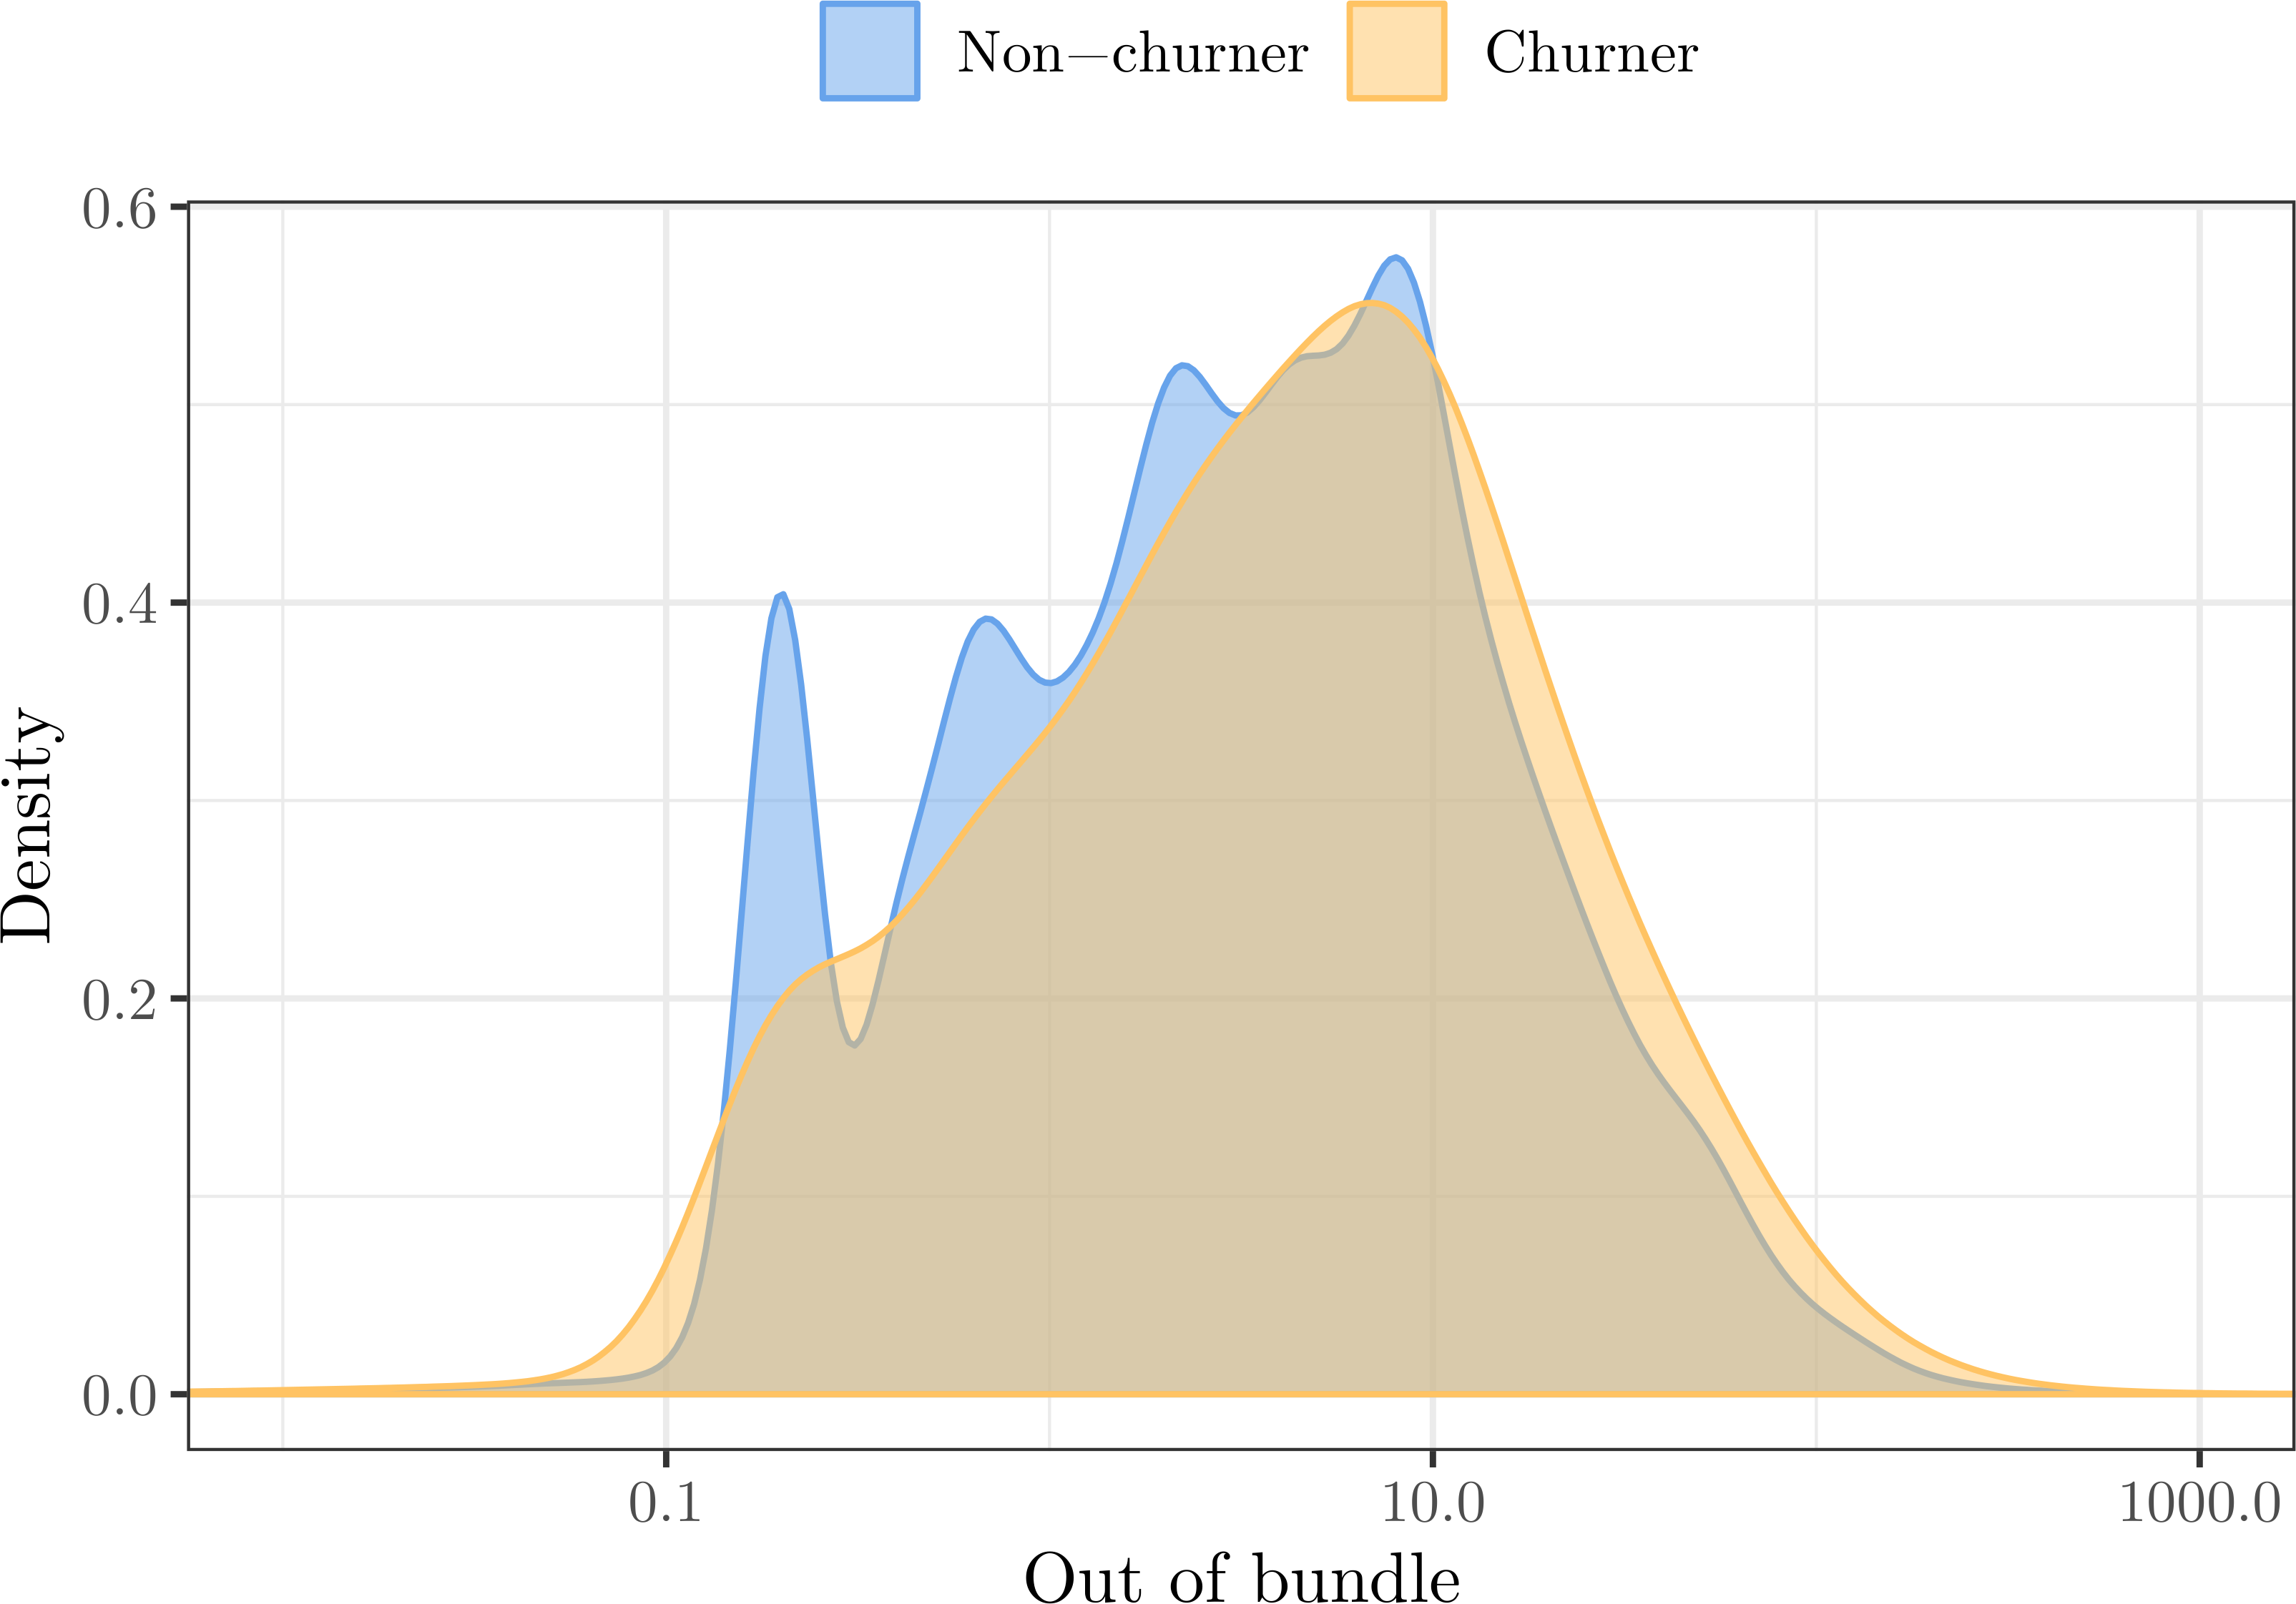
\includegraphics[width=0.9\linewidth]{figures/oob.png}
	\caption{Out-of-bundle amount (extra amount to pay on top of the usual
	invoice), in logarithmic scale.}
	\label{fig:oob}
\end{figure}

The importance of the tenure (the duration of the current subscription) is shown
in figure \ref{fig:tenure}. This graph displays the density of clients as a
function of the tenure. For confidentiality reasons, the scale of the x-axis is
hidden. The curve can be divided into two components: new customers and
long-term customers. One can clearly observe that proportionally more churners
are present in the first component than in the second. This indicates that
long-term clients tend to churn less, whereas new clients are much riskier.

\begin{figure}
    \centering
	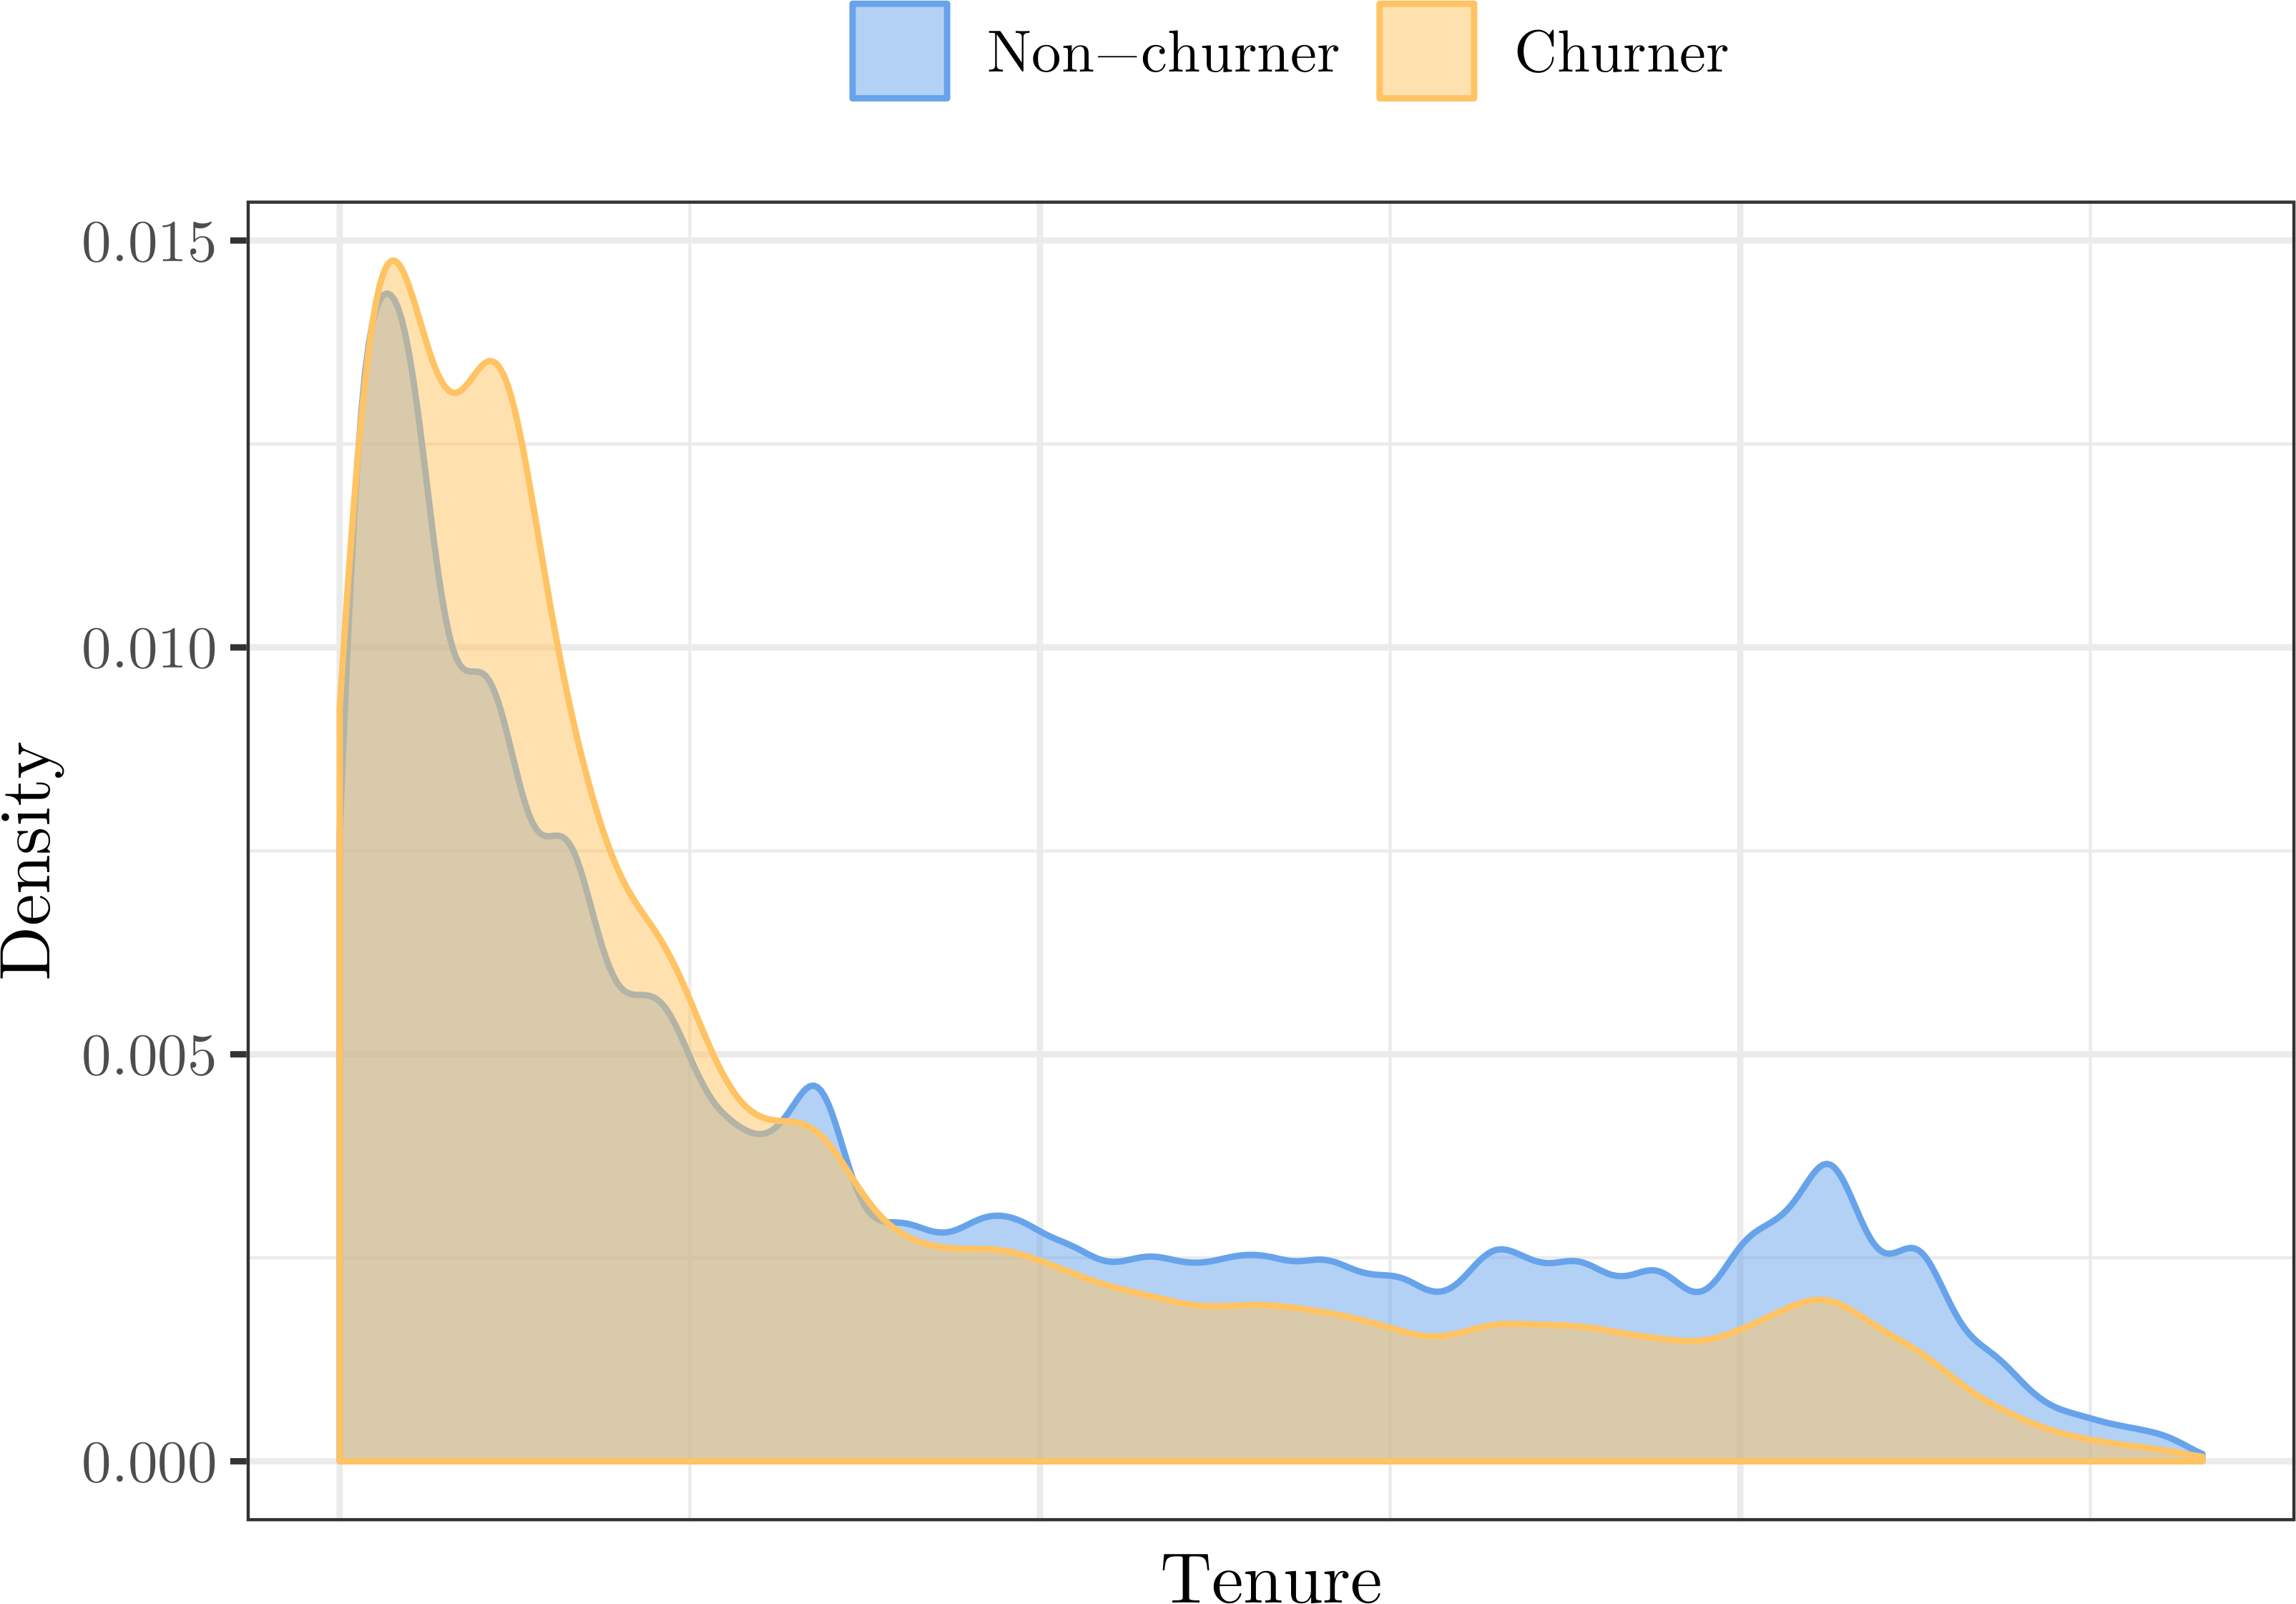
\includegraphics[width=0.9\linewidth]{figures/tenure.png}
	\caption{Tenure (time spent without churning so far) for churners and
	non-churners.}
	\label{fig:tenure}
\end{figure}

Figures \ref{fig:binary} and \ref{fig:categorical} show the distribution of two
discrete categorical variables. The first variable, R14, is a binary flag
related to revenues and is slightly less often true among churners. The second
variable, H8, is a categorical variable related to hardware and takes 8
different values. The churn rate varies moderately depending on the value of
this variable.

\begin{figure}
    \centering
    \begin{minipage}{.45\textwidth}
    	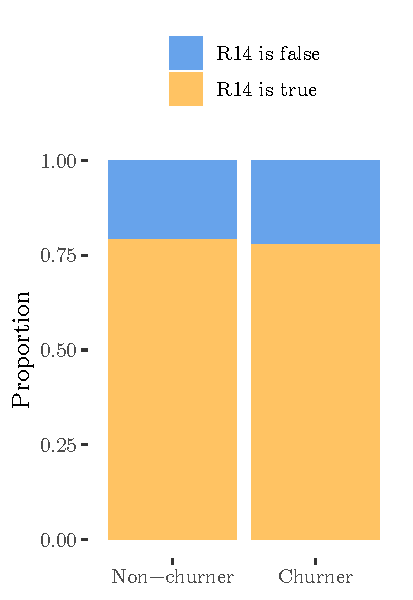
\includegraphics{figures/binary.pdf}
    	\caption{Distribution of a binary variable related to revenues, R14, for
    	churners and non-churners.}
    	\label{fig:binary}
    \end{minipage}
    \hspace{0.05\textwidth}
    \begin{minipage}{.45\textwidth}
    	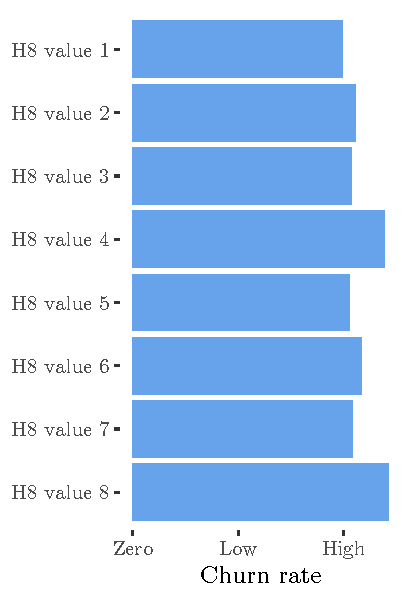
\includegraphics{figures/categorical.pdf}
    	\caption{Distribution of churn rate depending on a categorical variable
    	related to hardware, H8.}
    	\label{fig:categorical}
    \end{minipage}
\end{figure}


We demonstrate the interaction between two categorical variables in figure
\ref{fig:binary_payment_responsible}. The horizontal axis indicates whether a
customer has a cable connection, and the vertical axis denotes the payment
responsible flag. This flag is set to false only when someone else pays the bill
of the customer, such as a parent. Most customers of Orange Belgium do not have
a cable connection, and are responsible for the payment, as indicated by the
radius of the spots. The color of the spots indicates the churn rate, with a
lighter color denoting a higher probability of churn. The area is proportional
to the number of clients in each category. The impact of both binary variables
appears clearly, with a significant difference of churn rate between the two
extrema. Once again, the precise value of churn rate cannot be disclosed.


\begin{figure}
    \centering
	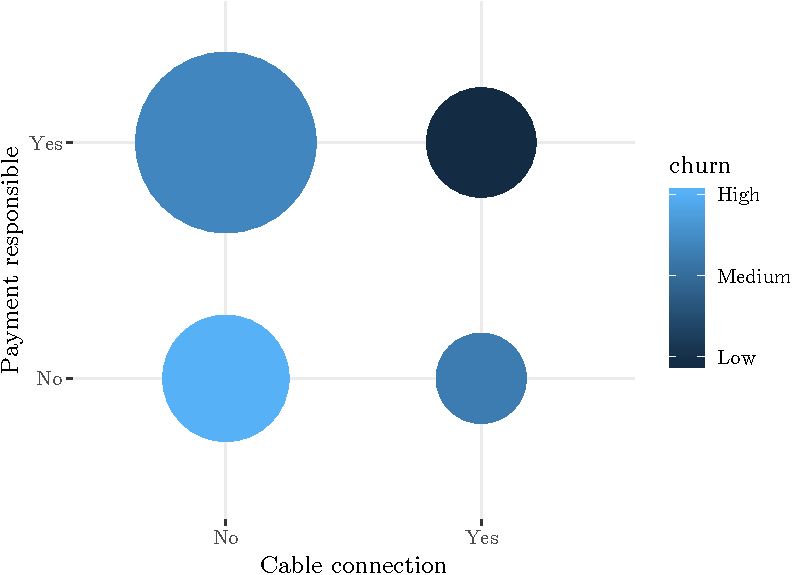
\includegraphics[width=0.9\linewidth]{figures/flagcable_payment_responsible.pdf}
	\caption{Interaction between cable connection and payment responsible. A
	customer is not responsible for payment if someone else (e.g. a parent) pays
	the invoice in her stead. The color of the spots denotes the churn rate,
	whereas its area denotes the number of customers.}
	\label{fig:binary_payment_responsible}
\end{figure}


A principal component analysis (PCA) demonstrates the important overlap between
churners and non-churners (figures \ref{fig:pca_1_2} and \ref{fig:pca_1_2}). The
blue corresponds to non-churners, while the orange and yellow represent
the churners respectively in the validation and the test set. We explain how the
test set and the validation set are partitioned in section
\ref{sec:churn_data_seg}. The ellipses represent the contour lines of
covariance, that is, the set of points at a Mahalanobis distance of 1 from the
mean in each set. The mean of each set is pictured as a dot in the center of the
figure. A large overlap between the population
of churners and non-churners appears clearly. Also, the standard deviation is larger in the
population of churners, reflecting the interpretation that churn is associated
with larger values for the out-of-bundle amount, number of calls, data usage,
etc.

\begin{figure}
    \centering
    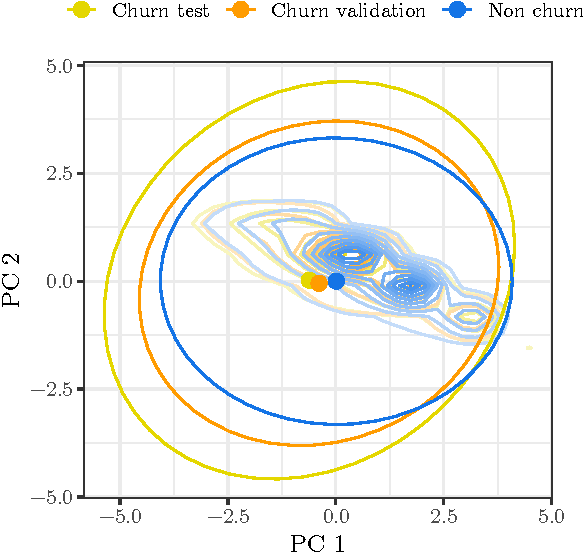
\includegraphics[width=0.63\linewidth]{figures/pca_1_2.pdf}
    \caption{Projection of the dataset onto the first two principal components.
    The ellipses show the set of points at a Mahalanobis distance of 1 from the
    mean of each group, which are represented by a dot.}
    \label{fig:pca_1_2}
\end{figure}

\begin{figure}
    \centering
    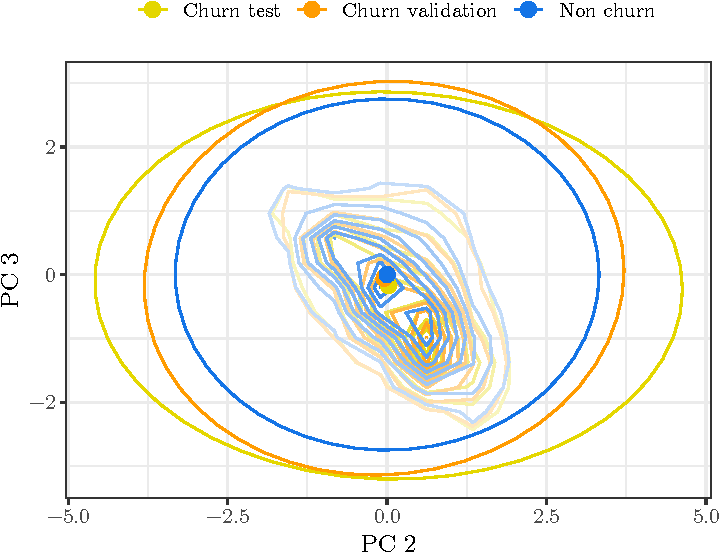
\includegraphics[width=0.8\linewidth]{figures/pca_2_3.pdf}
    \caption{Projection of the dataset onto the second and third principal
    components. The ellipses show the set of points at a Mahalanobis distance of
    1 from the mean of each group, which are represented by a dot.}
    \label{fig:pca_2_3}
\end{figure}

This data analysis demonstrates the high complexity of the churn prediction
problem. No unique variable allows to unambiguously predict churn since there is
a significant overlap between the population of churners and non-churners.
Informative variables such as the tenue (figure \ref{fig:tenure}) or the
out-of-bundle amount (figure \ref{fig:oob}) allow to increase or decrease the
confidence into churn only marginally. A large number of variables must be used
in conjunction in order to achieve decent predictive performances. Moreover, we
have no guarantee that the set of available variables are sufficient, it is
easily conceivable that unknown factors, such as a promotion launched by a
concurrent company, play a significant role.

\section{Data preparation}
\label{sec:data_pre}

The data preparation is of a sequence of steps.

\begin{description}

	\item[Unknown values preprocessing] The original data uses various means to
	specify an unknown categorical value. For example, an unknown previous
	tariff plan is either represented by an empty string, the string
	\texttt{"u"}, the string \texttt{"null"} or a null value. This preprocessing
	step replaces these various encodings by a unique one. Also, missing values
	in continuous variables are either replaced by zero or by the mean of the
	variable, depending on the semantics (e.g. null data usage is replaced by
	zero, whereas missing age is replaced by the average age in the dataset).

	\item[Date encoding] Some fields are represented by a date, such as the last
	contract change, the date of contract activation, or the churn date. These
	fields are converted to the number of days between the first day of the
	month of the dataset entry and the field value. For example, let us consider
	an entry about the activity of a customer in January 2019. Say this entry
	contains a field with the contract activation date, with value \texttt{"20
	December 2018"}. This field is converted to an integer value of 12,
	since there are 12 days between 1st January 2019 and 20 December 2018.

    \item[Clustering of character strings] There are three character string
    variables, representing the current and the previous tariff plan, and the
    manufacturer of the customer's device. These three variables could be
    considered as categorical variables, but the high number of different values
    would make this difficult to implement. We alleviate this difficulty by
    clustering all the different values into a small number of groups. In the
    case of the two tariff plan variables, this corresponds to the different
    tariff plan options (\emph{Hummingbird}, \emph{Koala}, \emph{Eagle}, etc).
    For the device manufacturer, we keep the 7 most common values, and we
    replace all the less frequent values by "Other".

	\item[Difference and ratio columns] For each numerical field representing a
	quantity that can change from month to month (such as the total duration of
	calls, or the mobile data usage), we create 2 additional fields. They
	contain the difference and the ratio of the value of the field with that of
	the same field the previous month. This hopefully gives the model an
	indication of the customer's behavior evolution over the course of the last
	month. 41 variables are suitable for this operation, therefore increasing
	the number of variables up to 155. If no data is available for the previous
	month (such as for the first month of data), the differences are set to 0
	and the ratios are set to 1. In order to reduce computation time, not all
	experiments use these new columns, as discussed in the next section. This
    augmented dataset is named ``SIM only $\Delta$'' thereafter.

	\item[Normalization] The data is normalized to obtain zero mean and unit
	variance. Even though the only models being used are random forests, which
	are not sensitive to linear scaling of its input variables, this step is
	kept in the event that we would have tried another model requiring
	normalization (such as support vector machine or neural networks). This
	preprocessing step is also useful for sensitivity analysis, where we add a
	small value to a variable and observe the difference in the predictions of
	the model. In this case, a normalized dataset allows to use the same
	difference value for all variables.

    \item[Target variable] The last step is to create a binary target variable
    from the churn date. It is defined to be true if and only if the date of
    churn is in the two months following the current data entry. If the churn
    date is in the current month or before, then the entry is discarded, for two
    reasons. Firstly, the information contained in these entries is incomplete.
    Secondly, this data is not relevant for churn prediction, as we wish to
    predict churn at least a few days in advance. It is not interesting to learn
    patterns exhibited by clients that will churn the next day, as there is
    probably no longer any hope of successful retention. If the churn date is
    not given, or if it is more than two months after the month of the data
    entry, the churn variable is set to false. This process is pictured in
    figure \ref{fig:data_separated}. The choice of the time threshold is
    dependent on the business application. A lower threshold focuses on
    short-term churn, whereas a larger threshold enables to predict churn from
    further in the future. Models already in use at Orange Belgium consider a
    time period of two months, we therefore use this value in order to enable
    the comparison of our results with production models.

\end{description}

\begin{figure}
    \centering
	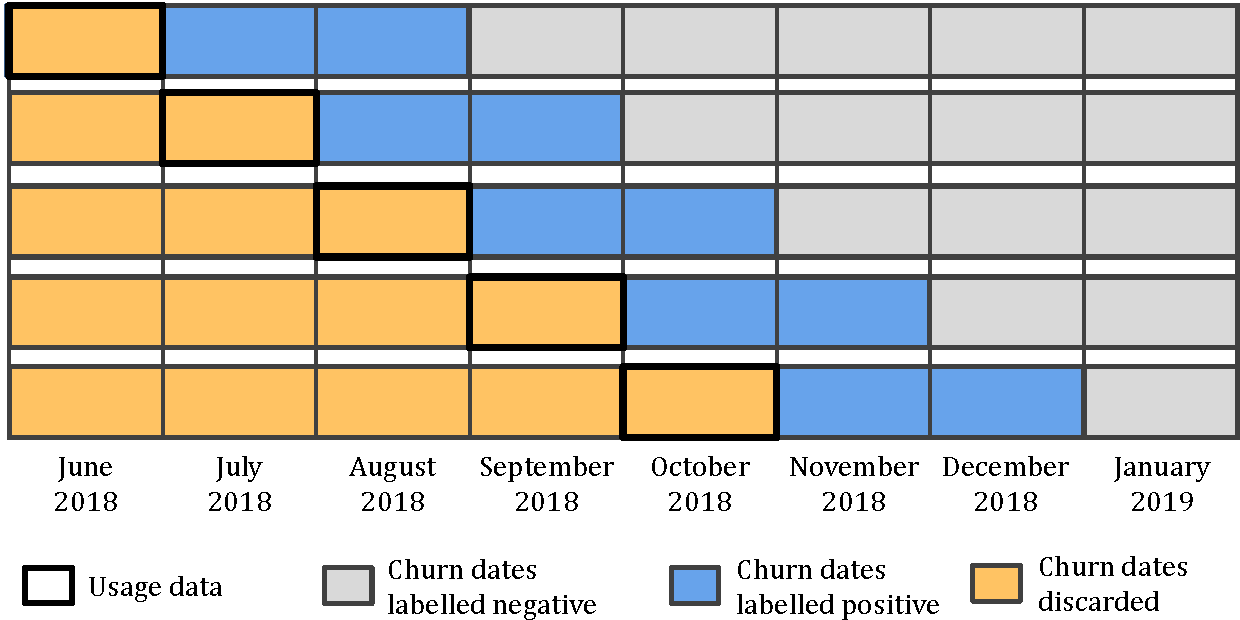
\includegraphics[width=0.9\linewidth]{figures/data_range.pdf}
	\caption{Outline of the target variable assignment. The dataset is separated
	in 5 months and each data entry in each month is labeled as churner if the
	churn date is given and less than two months ahead.}
	\label{fig:data_separated}
\end{figure}

\section{Experiments}
\label{sec:churn_exp}

\subsection{Scope}

The experiments on predictive modeling consist in the training of predictive
models on the data described in the previous sections, and an assessment of
their performance. Three datasets are derived from the output of the
preprocessing step: one containing the loyalty contracts, one containing the SIM
only contracts, and one containing the SIM only contracts with difference and
ratio variables (called SIM only $\Delta$). We evaluate the impact of

\begin{enumerate}
    \item variable selection, based on the feature importance provided by
    trained random forest models;
    \item the addition of difference and ratio variables;
    \item the type of contract (SIM only vs. loyalty).
\end{enumerate}

The high computational cost of the model training on such a large dataset does
not allow to test all the possible configurations of these three parameters. We
limited the number of selected variables to 20, 30 or all variables. Also, we do
not explore the difference variables for loyalty contracts. These
combinations of parameters yield 9 different experiment configurations.


\subsection{Data segmentation}
\label{sec:churn_data_seg}

In each configuration, the corresponding dataset is split into a training and a
test set. The training set comprises the first 4 months of data and the test set
comprises only the last month, as pictured in figure
\ref{fig:experiment_diagram}. Separating by months allows for a potential
concept drift from the training set to the test set (i.e. a change in the
typical behavior exhibited by churners). We perform a $k$-fold cross-validation
on the training set in order to provide an indication of the performance of our
model on the training data. We set $k=3$, as a compromise between statistical
significance and computation time. The difference in prediction accuracy between
the validation set and the test set indicates how much patterns learned on the
training set are still relevant for the next month. This indicates whether
training has to be repeated each month as new data arrives from the customers.
Note that when testing the model on the test set, a new model is trained on the
whole training set.

\begin{figure}
    \centering
	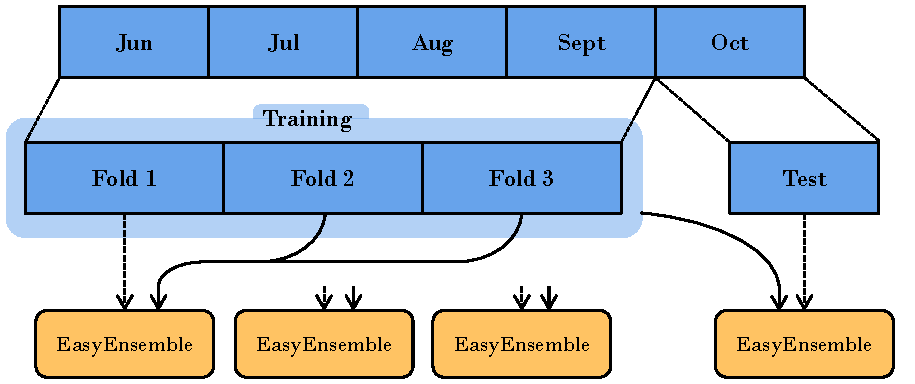
\includegraphics[width=0.9\linewidth]{figures/experiment_diagram.pdf}
	\caption{Outline of the data repartition between training and test set, with
	a 3-fold cross-validation on the training set. Dotted arrows indicate
	testing and solid arrows indicate training. Arrows for two of the three
	validation models are not shown.}
	\label{fig:experiment_diagram}
\end{figure}

\subsection{Class balancing}

In order to counteract the sheer prominence of non-churners in the dataset, we
need to use class balancing. We use the EasyEnsemble algorithm, presented in
section \ref{sec:sota_balancing}. It consists in training different models on
the whole set of positive instances, and on a randomly selected set of negative
instances. The number of negative instances is chosen so that the ratio between
the two classes is even. In all experiments, the EasyEnsemble is set to use 10
random forest models.

\subsection{Evaluation measure}

The performance of the different models is evaluated using three different
measures: the lift curve, the receiver operating characteristic (ROC) curve, and
the precision-recall (PR) curve. While the ROC curve and the PR curve are widely
used in the machine learning literature, the lift curve is of more practical
interest in evaluating churn prediction. Since a customer churn retention
campaign focuses on a limited amount of customers, the lift curve allows
observing the expected performance of the model as the number of customers
included in the campaign varies. From the ROC and PR curves, we derive the area
under the ROC curve (AUROC), the area under the PR curve (AUPRC) and the lift at
different thresholds (1\%, 5\%, and 10\%).

We argue that the most sensible cost evaluation functions are the maximum profit
criterion (MPC) and the expected maximum profit criterion (EMPC)
\parencite{verbeke2012new, verbraken2013novel}. These take into account the
different costs and benefits yielded by a retention campaign and provide the
decision threshold that should be applied to maximize the profit given the
probability distribution output by a prediction algorithm. This process
formalizes the intuition behind the lift criterion that the prediction algorithm
should focus on reducing false positives, since the retention campaign is not
able to reach each and every potential churner. Despite the relevance of this
approach under a profit-centric point of view, we are not able to use this
evaluation measure in our study. This is caused by the necessity to evaluate
different costs and benefits parameters, such as the cost of reaching a
customer, the probability that a customer accepts an incentive, the benefit if
the customer accepts it, etc. The evaluation of these parameters is a
time-consuming process and is outside of the scope of our work.


\subsection{Sensitivity analysis}
\label{sec:churn_sens}

The impact of variables on churn prediction is derived in two different ways.
The first corresponds to the variable importance output by the random forest
models. Each random forest calculates a score for each variable by measuring how
much the prediction accuracy decreases when all the values of this variable are
randomly permuted. The decrease in accuracy is calculated over the out-of-bag
samples in each tree. This permutation cancels out any statistical dependency
between this variable and the target variable, giving an estimate of the
importance of the variable in the trained model. Note that if two variables
share the same information about the target (for example by being highly
correlated), the importance of both of these variables will be less than if only
one were present. This is due to the fact that the two variables are equally
likely to be chosen when splitting nodes in a tree, therefore reducing the
impact of the removing one of the two variables when computing the importance.

This measure of importance allows to understand the predictive power of each
variable but does not indicate the directionality of its impact on the
predictions. We address this issue by constructing, for each variable $X_i$, an
alternate training set identical to the original one, but where a value equal to
one standard deviation $\sigma_{X_i}$ is added to each instance of the variable
$X_i$. A second shifted dataset is also constructed by subtracting instead of
adding the standard deviation. Then, the average predicted probability of churn
is computed for both the original training set and the shifted one, and the
difference between the two average probabilities is taken. This difference
indicates the impact of the variable on the predictions. For example, a
predicted churn probability lower for the training set where a standard
deviation is added to the tenure variable indicates that longer-standing
customers are associated with less churn. Note that we use in this experiment
the normalized dataset so that adding a standard deviation amounts to adding 1
to the instances of the variable.

\section{Results}

\begin{table}
    \centering
    \begin{tabular}{lrrrrrrrrr}
        \toprule
        & \multicolumn{3}{c}{\textbf{SIM only}}
        & \multicolumn{3}{c}{\textbf{SIM only $\Delta$}}
        & \multicolumn{3}{c}{\textbf{Loyalty}} \\
        \cmidrule(l){2-4} \cmidrule(l){5-7} \cmidrule(l){8-10}
        & \textbf{20} & \textbf{30} & \textbf{All} & \textbf{20} & \textbf{30} &
        \textbf{All} & \textbf{20} & \textbf{30} & \textbf{All} \\
        \midrule

        AUROC        & 0.66 & \underline{0.73} & \underline{0.73} & 0.72 &
        \underline{0.73} & 0.69 & 0.74 & \underline{0.76} & \underline{0.76} \\

        AUPRC        & 0.05 & \underline{0.10} & \underline{0.10} &
        \underline{0.10} & \underline{0.10} & 0.08 & 0.15 & \underline{0.19} & 0.18 \\

        Lift at 10\% & 2.25 & 3.34 & 3.41 & 3.27 & \underline{3.42} & 3.03 &
        2.96 & \underline{3.40} & 3.30 \\

        Lift at 5\%  & 2.64 & 4.49 & \underline{4.68} & 4.48 & 4.67 & 4.09 &
        3.51 & \underline{4.22} & 4.02 \\

        Lift at 1\%  & 4.29 & 9.20 & 9.53 & \underline{10.09} & 9.95 & 7.67 &
        4.66 & \underline{6.65} & 6.16 \\
        \bottomrule
    \end{tabular}
    \caption{Summary of the results of prediction experiments on the test set.
    Highest values for each type of contract and for each evaluation measure are
    underlined for the test set.}
    \label{tab:results}
\end{table}

This section shows the results of the predictive experiments. Figures
\ref{fig:lift_simo} to \ref{fig:pr_loy} are performance curves for the three
different datasets. Each plot contains a curve for both validation and test
sets, and for the configurations where we select 20, 30 or all of the variables.
This amounts to a total of 6 curves per plot. As explained in section
\ref{sec:churn_exp}, the validation is done on the 4 first months of data,
whereas the test set corresponds to the last month. Figures \ref{fig:lift_simo}
to \ref{fig:lift_loy} show the lift curves, figures \ref{fig:roc_simo} to
\ref{fig:roc_loy} show the ROC curves, and figures \ref{fig:pr_simo} to
\ref{fig:pr_loy} show the precision-recall curves. A summary of the results is
given in table \ref{tab:results}. The lift at different thresholds, the area
under the ROC curve, and the area under the precision-recall curves are reported
for the test set. Table \ref{tab:results_valid} provides the same information
for the predictions on the validation set. The impact of the different
experimental parameters on predictive performance is discussed in the next
sections.

In this section, numerical scores associated with variables are displayed as
horizontal bar plots. The colors of the bars correspond to the
categories of variables presented in section \ref{sec:churn_data}:

\begin{itemize}
    \item[\color{themeyellow}$\blacksquare$] \setulcolor{themeyellow}\ul{Subscription}
    \item[\color{themeblue}$\blacksquare$] \setulcolor{themeblue}\ul{Calls and messages}
    \item[\color{darkerblue}$\blacksquare$] \setulcolor{darkerblue}\ul{Mobile data usage}
    \item[\color{themepurple}$\blacksquare$] \setulcolor{themepurple}\ul{Revenue}
    \item[\color{darkerorange}$\blacksquare$] \setulcolor{darkerorange}\ul{Customer hardware}
    \item[\color{themeorange}$\blacksquare$] \setulcolor{themeorange}\ul{Socio-demographic}
\end{itemize}

\begin{figure}
    \centering
    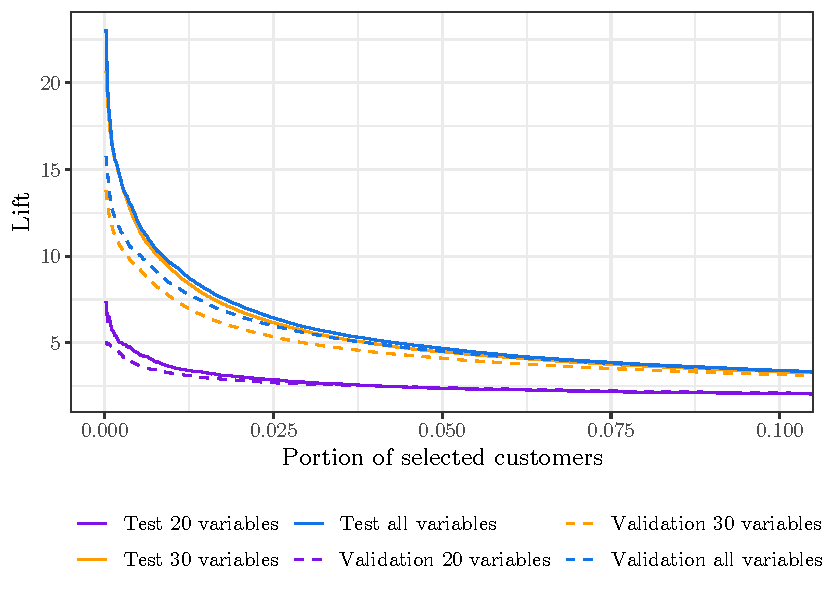
\includegraphics[width=0.9\linewidth]{figures/lift_simo.pdf}
    \caption{Lift curve for SIM only}
    \label{fig:lift_simo}
\end{figure}

\begin{figure}
    \centering
    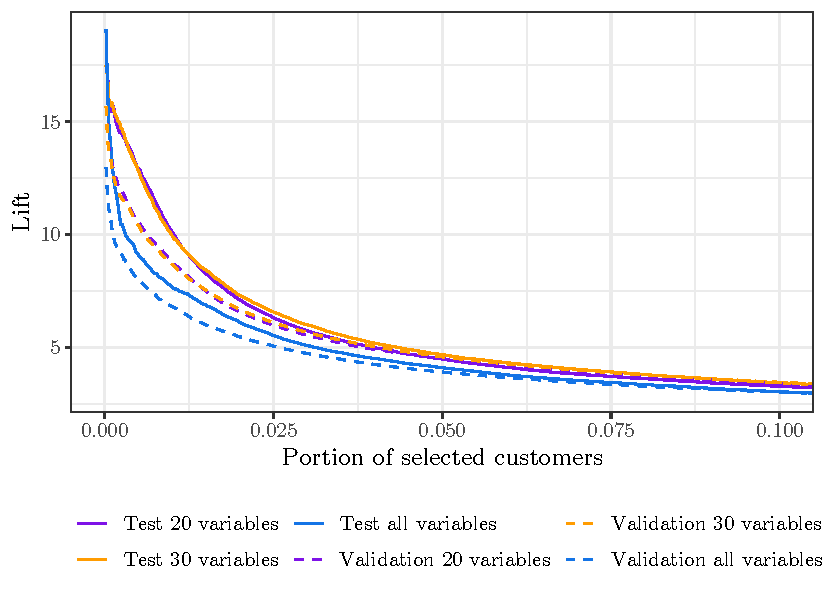
\includegraphics[width=0.9\linewidth]{figures/lift_simo_diff.pdf}
    \caption{Lift curve for SIM only with difference and ratio variables}
    \label{fig:lift_simo_diff}
\end{figure}

\begin{figure}
    \centering
    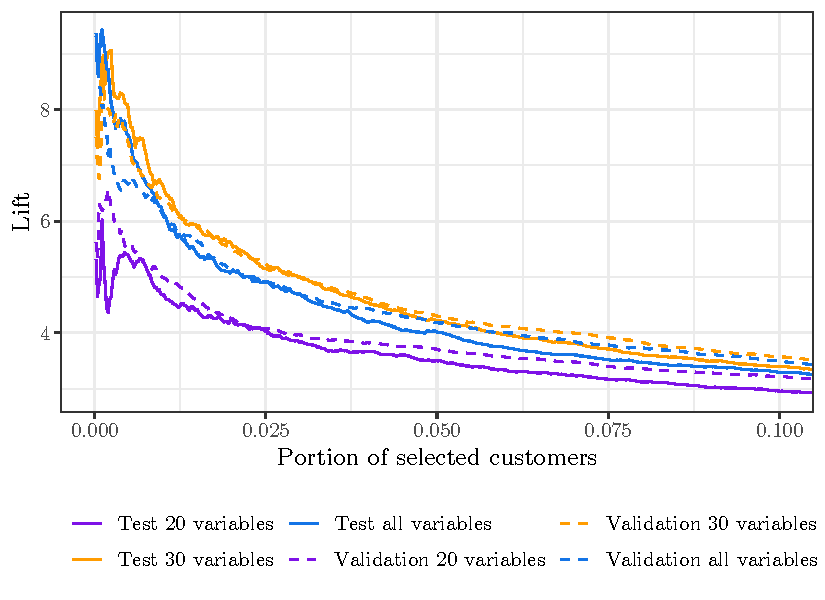
\includegraphics[width=0.9\linewidth]{figures/lift_loy.pdf}
    \caption{Lift curve for loyalty}
    \label{fig:lift_loy}
\end{figure}

\subsection{Number of variables}

The number of variables has an influence on the prediction accuracy, and this
impact depends on the dataset under consideration. Recall that in each
configuration, the selected variables are chosen according to the variable
importance given by the random forests trained on the whole training set. In the
case of the SIM only dataset (figures \ref{fig:lift_simo}, \ref{fig:roc_simo}
and \ref{fig:pr_simo}), selecting only 20 variables decreases drastically the
performance. Selecting 30 variables achieves performances almost as good as
selecting the whole set of 73 variables.

\begin{figure}
    \centering
    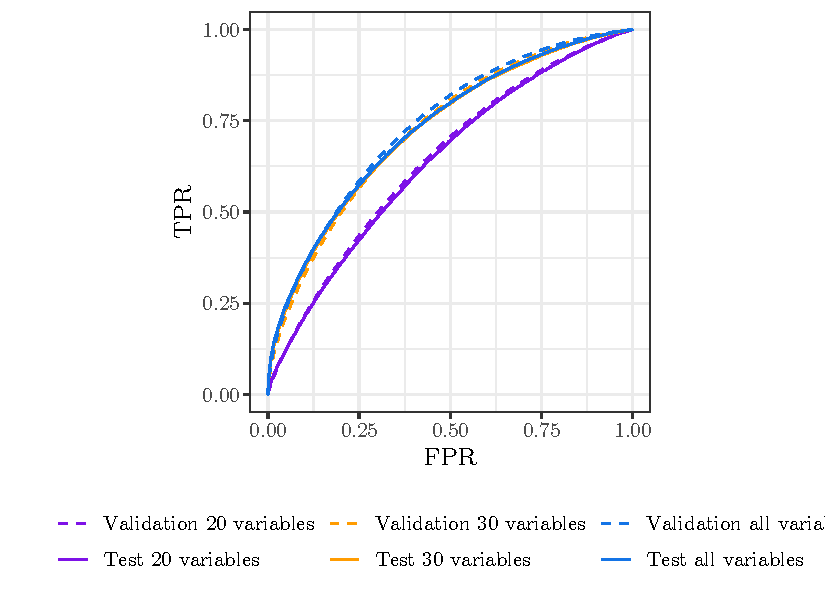
\includegraphics[width=0.9\linewidth]{figures/roc_simo.pdf}
    \caption{ROC curve for SIM only.}
    \label{fig:roc_simo}
\end{figure}

For the SIM only $\Delta$ dataset, a lower number of variables is beneficial for
performance. As shown in figures \ref{fig:lift_simo_diff},
\ref{fig:roc_simo_diff} and \ref{fig:pr_simo_diff}, selecting all variables
appears to be detrimental to the accuracy, whereas choosing between 20 or 30
variables does not make a significant difference. This might be caused by the
additional variables that add more noise than useful information for the random
forests. It is interesting to note that selecting the top 20 variables when
considering the SIM only $\Delta$ dataset provides much better accuracy than
selecting the top 20 variables in the original dataset. As shown in figure
\ref{fig:var_imp_simo_diff_decrease_accuracy}, the 20 most important variables
in the SIM only $\Delta$ dataset do not even include any difference or ratio
variable. The difference between the top 20 most important variables is as
follow:

\begin{itemize}
    \item SIM only $\Delta$ includes the number of contracts, the age, and a
    variable on data usage, whereas SIM only does not;
    \item SIM only includes the device manufacturer, the previous tariff plan,
    and two other variables on data usage, whereas SIM only $\Delta$ does not.
\end{itemize}

\begin{figure}
    \centering
    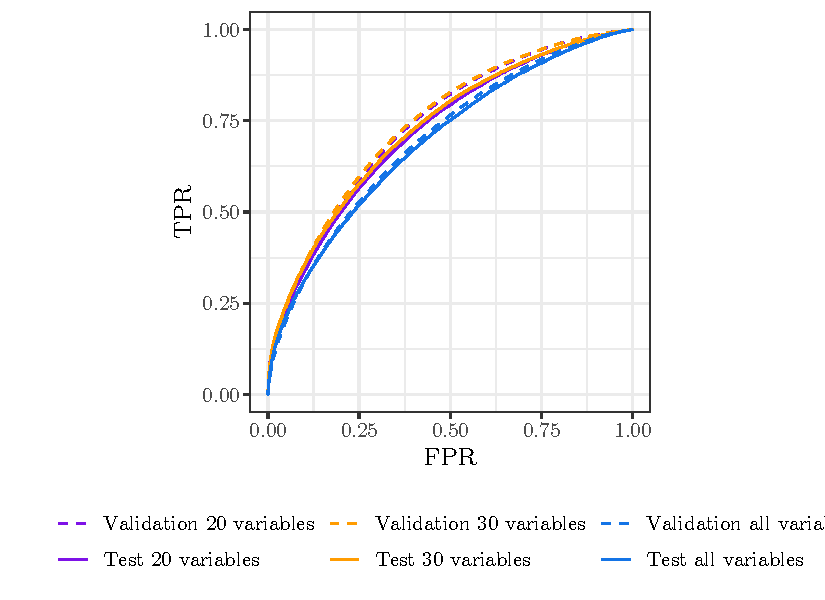
\includegraphics[width=0.9\linewidth]{figures/roc_simo_diff.pdf}
    \caption{ROC curves for SIM only with difference and ratio variables.}
    \label{fig:roc_simo_diff}
\end{figure}

The large difference in accuracy between these two configurations must be caused
by this difference in the selected variables, since all other variables and all
other experiment parameters are identical.

When considering the loyalty dataset, selecting 30 variables instead of the
whole set of 73 variables is marginally beneficial on low thresholds (less than
0.1). On the overall space of thresholds, the difference is not significant, as
indicated in table \ref{tab:results} with the AUROC and the AUPRC. However,
selecting only 20 variables is clearly detrimental.

\begin{figure}
    \centering
    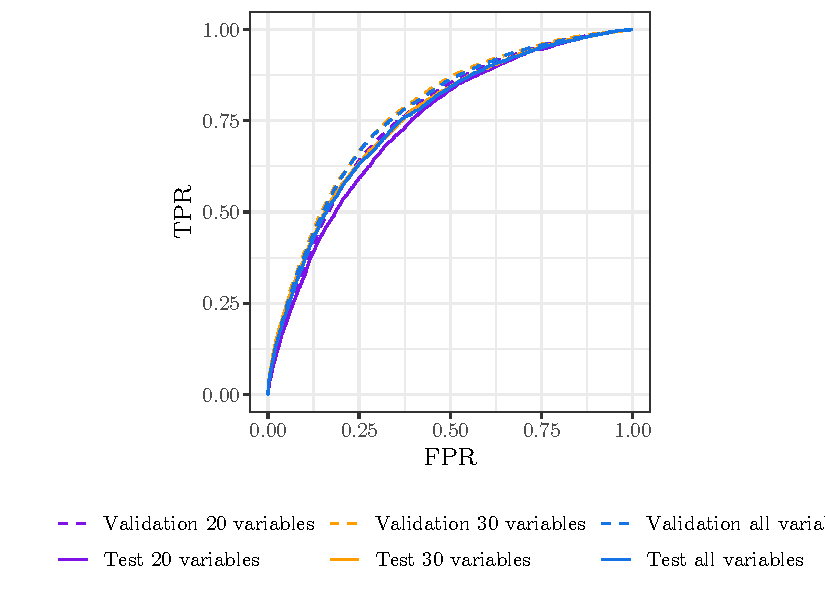
\includegraphics[width=0.9\linewidth]{figures/roc_loy.pdf}
    \caption{ROC curves for loyalty.}
    \label{fig:roc_loy}
\end{figure}

\subsection{Difference and ratio variables}

The difference and ratio variables do not have a positive impact on performance.
Indeed, the best performance achieved on the SIM only $\Delta$ dataset are
obtained by limiting the number of variables to 20 or 30. The variables being
selected in these cases do not include any of the difference and ratio
variables. If all variables are used, the performance of the random forests
decreases significantly, as shown in figures \ref{fig:lift_simo_diff},
\ref{fig:roc_simo_diff}, \ref{fig:pr_simo_diff}, and table \ref{tab:results}.
Moreover, the memory usage of this dataset is much higher than that of the
original dataset, thus complicating the training process.

\begin{figure}
    \centering
    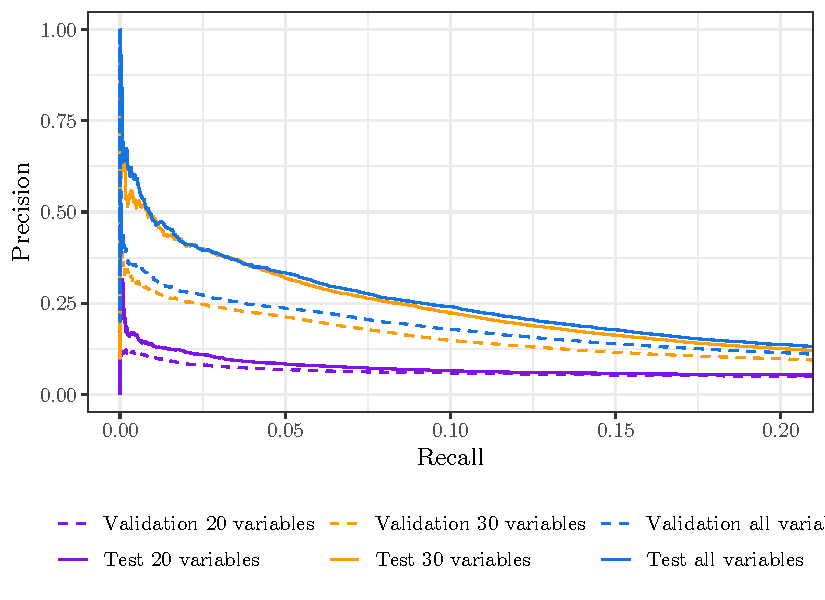
\includegraphics[width=0.9\linewidth]{figures/pr_simo.pdf}
    \caption{Precision-recall curves for SIM only.}
    \label{fig:pr_simo}
\end{figure}

\begin{figure}
    \centering
    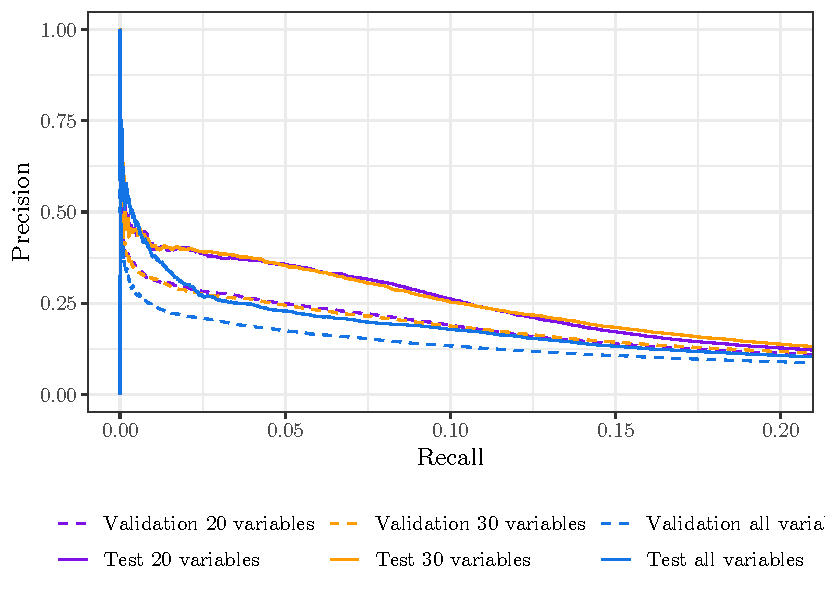
\includegraphics[width=0.9\linewidth]{figures/pr_simo_diff.pdf}
    \caption{Precision-recall curves for SIM only with difference and ratio
    variables.}
    \label{fig:pr_simo_diff}
\end{figure}

\begin{figure}
    \centering
    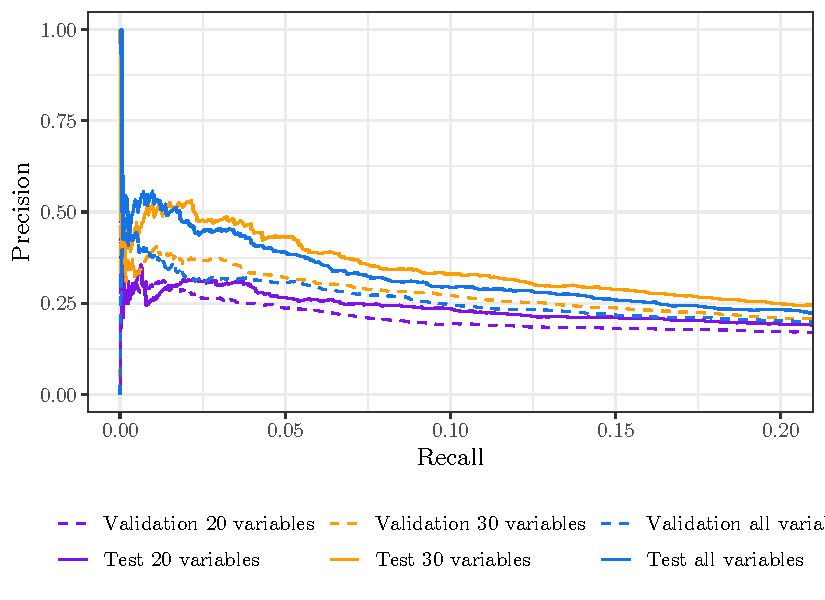
\includegraphics[width=0.9\linewidth]{figures/pr_loy.pdf}
    \caption{Precision-recall curves for loyalty.}
    \label{fig:pr_loy}
\end{figure}

\subsection{Generalization performances}

The generalization abilities of the trained models are evaluated by comparing the
accuracy on the validation set and on the test set. On the lift curves and on
the precision-recall curves, it appears that for all configurations, the
performance on the test set is better than on the validation set. Bear in mind
that on these curves, only a small fraction of the threshold space is
represented, whereas the ROC curves show all possible decision thresholds. This
observation implies that customers with a very high probability of churn are
proportionally more numerous in the test set than in the validation set. It is
illustrated in figures \ref{fig:pca_1_2} and \ref{fig:pca_2_3}, where the
ellipse of covariance of the test set is larger than that of the validation set.
This suggests that, in the test set, there are more churners with very high
values for variables having a large standard deviation. This probably
corresponds to the bill shock effect discussed in section \ref{sec:churn_data}:
a large ``out of bundle'' amount, caused by large data consumption, increases
the probability of churn. In this case, the bill shock is more pronounced in
the test set, explaining the improvement in predictions.

The performance measures on the validation set are summarized in table
\ref{tab:results_valid}. When we compare the lift at low thresholds in table
\ref{tab:results}, it is clear that the model manifests worse performance on the
validation set than on the test set. However, it is not the case for the AUROC
and the AUPRC, which take into account the whole space of decision threshold,
and not only the riskiest customers. We can conclude that our model has been
trained on a training set where the overlap between churners and non-churners is
more important than on the test set. The model thus generalizes well, and even
perform better on unseen data in our case due to a lucky domain shift.

\begin{table}
    \centering
    \begin{tabular}{lrrrrrrrrr}
        \toprule
        & \multicolumn{3}{c}{\textbf{SIM only}}
        & \multicolumn{3}{c}{\textbf{SIM only $\Delta$}}
        & \multicolumn{3}{c}{\textbf{Loyalty}} \\
        \cmidrule(l){2-4} \cmidrule(l){5-7} \cmidrule(l){8-10}
        & \textbf{20} & \textbf{30} & \textbf{All} & \textbf{20} & \textbf{30} &
        \textbf{All} & \textbf{20} & \textbf{30} & \textbf{All} \\
        \midrule
        AUROC & 0.64 & 0.73 & 0.74 & 0.74 & 0.74 & 0.70 & 0.76 & 0.78 & 0.77 \\
        AUPRC & 0.04 & 0.08 & 0.08 & 0.09 & 0.09 & 0.07 & 0.13 & 0.16 & 0.15 \\
        Lift at 10\%  & 2.10 & 3.16 & 3.39 & 3.39 & 3.44 & 3.01 & 3.22 & 3.57 & 3.50 \\
        Lift at  5\%  & 2.41 & 4.11 & 4.52 & 4.49 & 4.57 & 3.90 & 3.71 & 4.30 & 4.18 \\
        Lift at  1\%  & 3.24 & 7.58 & 8.36 & 8.80 & 8.67 & 6.79 & 5.00 & 6.37 & 6.11 \\
        \bottomrule
    \end{tabular}
    \caption{Summary of the results of prediction experiments on the validation
    set.}
    \label{tab:results_valid}
\end{table}

\subsection{Type of contract}

As indicated in table \ref{tab:results}, the models trained on loyalty perform
slightly worse than that of the SIM only datasets on small thresholds, but better
on larger thresholds. The AUROC is equal to 0.76 for loyalty, whereas the best
performing configuration for SIM only achieves an AUROC of 0.73. The AUPRC is
almost double, and this can be seen in figure \ref{fig:pr_loy}. The
precision is similar to that of the SIM only for low recall but decreases much
more slowly. It is still at approximately 0.25 when the recall is 0.2, whereas,
in the SIM only PR curves, the precision is already at 0.12 at this threshold.

Recall that there are fewer loyalty customers than SIM only, less confidence can
thus be given to the statistical results for loyalty, especially at low
thresholds. According to these results, the models trained on the loyalty
customers are slightly less efficient on small thresholds, but this is made up
for on larger thresholds. The increase in performance is probably due to the
more obvious churn patterns exhibited by loyalty customers. Indeed, most of the
churn in this population is due to the end of the mandatory period of the
subscription. This is reflected in figure
\ref{fig:var_imp_loy_decrease_accuracy}, where time-related variables are
prominent in variable importance. Given that we know when the mandatory part of
the customer's contract ends, the confidence of the model in the probability of
churn is increased compared to the SIM only case.

\subsection{Sensitivity analysis}

The results of sensitivity analysis are shown in figures
\ref{fig:var_imp_simo_decrease_accuracy} to \ref{fig:offset_1m}. Figures
\ref{fig:var_imp_simo_decrease_accuracy} to
\ref{fig:var_imp_loy_decrease_accuracy} show the variable importance given by
the random forest models. There is one plot per dataset, and in each plot, the
importance of each variable is averaged over the 10 models underlying the Easy
Ensemble meta-model. As discussed in the previous section, the most important
variables for the SIM only and the SIM only $\Delta$ datasets are almost
identical. They consist in a mix of socio-demographic variables (e.g. the
province), information about the tenure and the tariff plan of the customer, and
aggregate variables related to phone calls. The difference and ratio variables
are ranked fairly low for SIM only $\Delta$, the first one having a rank of 40
(not shown in figure \ref{fig:var_imp_simo_diff_decrease_accuracy}). On the
other hand, the selected variables for the loyalty dataset (figure
\ref{fig:var_imp_loy_decrease_accuracy}) are quite different. The tenure (first
and third variables) and other time-related variables on the subscription are
all important variables. Information relative to the type and time of
subscription is therefore important for predicting churn in loyalty contracts.
This is illustrated by the yellow color dominating the graph. Also, the age is
more important than for the SIM only dataset, as well as the variables U1, U2,
and U3, corresponding to data usage. This is consistent with an interpretation
of a younger and fickler customer base, consuming more data and more prone to
churn.

\begin{figure}
    \centering
    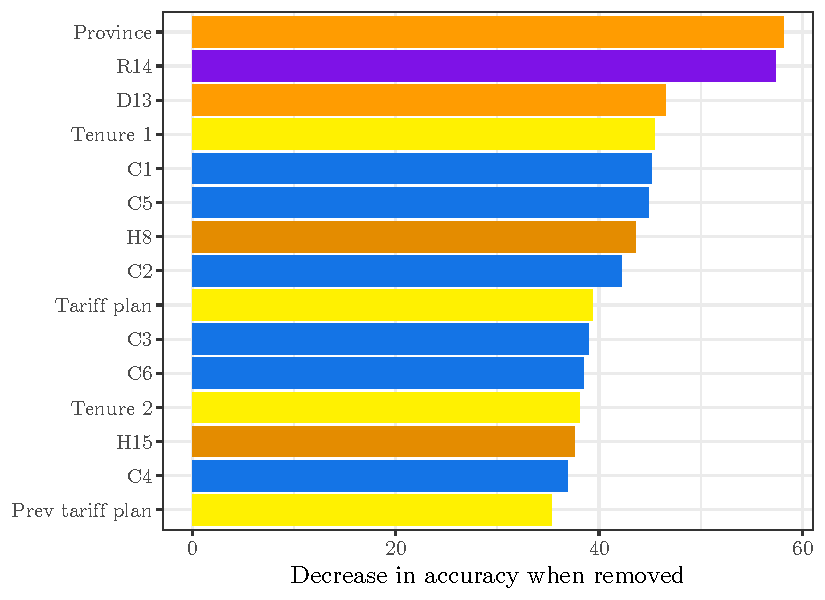
\includegraphics[width=0.9\linewidth]{figures/var_imp_simo_decrease_accuracy.pdf}
    \caption{Mean decrease in accuracy when a feature is removed for SIM only.}
    \label{fig:var_imp_simo_decrease_accuracy}
\end{figure}


Figures \ref{fig:offset_1p} and \ref{fig:offset_1m} display the shift in
predicted churn probability when a variable is offset by one standard deviation.
Figure \ref{fig:offset_1p} corresponds to an increase in the value of each
variable, whereas figure \ref{fig:offset_1m} corresponds to a decrease. The
tenure and the number of contracts have a symmetric effect: an observed increase
in their value reduces the probability of churn, and conversely. For the tenure,
this corresponds to the intuition that a newer customer is more prone to churn.
The number of contracts is a marker of commitment of a customer to Orange, and
the presence of this variable in both figures \ref{fig:offset_1p} and
\ref{fig:offset_1m} expresses that it has also a monotonic relation to churn
probability.


\begin{figure}
    \centering
    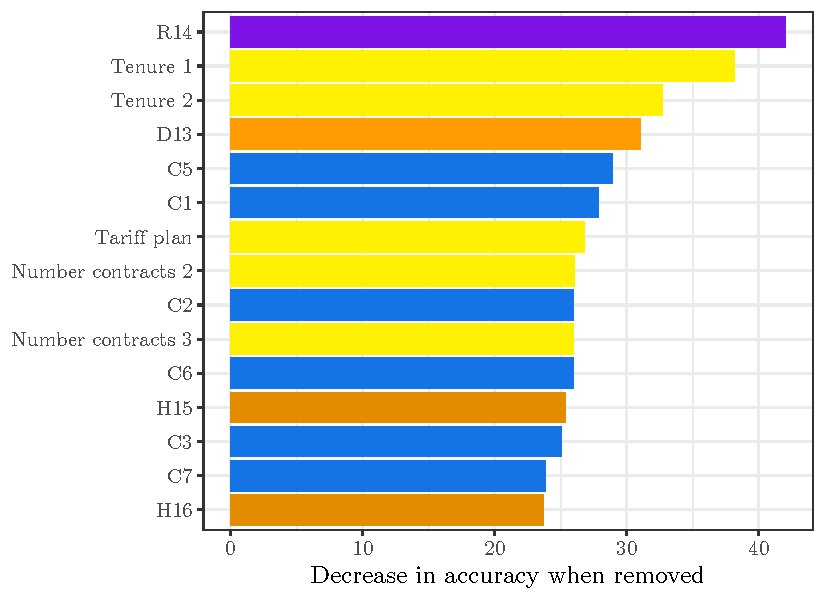
\includegraphics[width=0.9\linewidth]{figures/var_imp_simo_diff_decrease_accuracy.pdf}
    \caption{Mean decrease in accuracy when a feature is removed for SIM only
    with difference and ratio variables.}
    \label{fig:var_imp_simo_diff_decrease_accuracy}
\end{figure}


On the other hand, all other variables in this sensitivity analysis display a
non-linear relationship to predicted churn probability. This is remarkably
illustrated by the prominence of variables related to revenues in figure
\ref{fig:offset_1p}, colored in purple. These variables increase the predicted
probability of churn when they are increased, as expected by the bill shock
effect. However, they are absent from figure \ref{fig:offset_1m}, indicating
that a reduced bill is not associated with a reduced churn. It is worth mentioning
that the age is associated in both graphs with an increased risk of churn.
Consequently, any age far from the average age is associated with an increased
risk of churn.


\begin{figure}
    \centering
    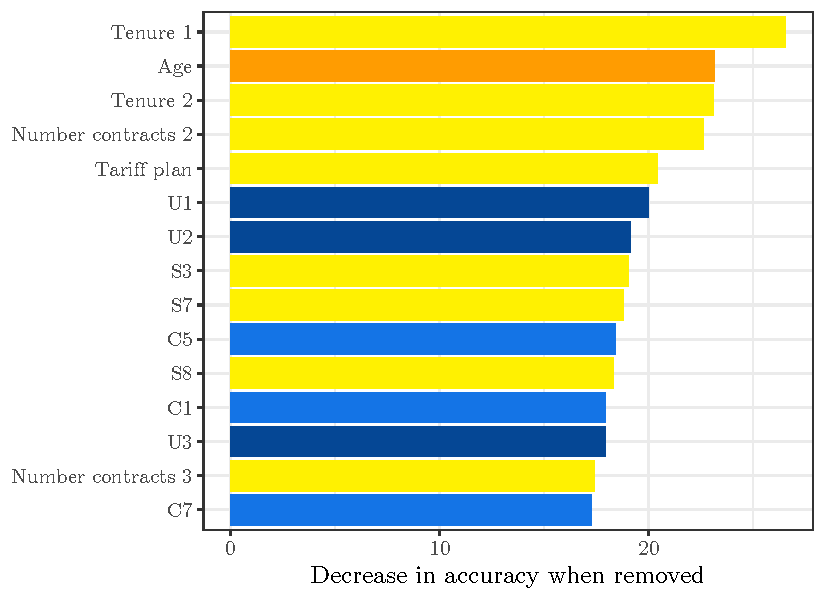
\includegraphics[width=0.9\linewidth]{figures/var_imp_loy_decrease_accuracy.pdf}
    \caption{Mean decrease in accuracy when a feature is removed for loyalty.}
    \label{fig:var_imp_loy_decrease_accuracy}
\end{figure}

Bear in mind that this analysis is solely indicating statistical associations
between the values of different variables and the predicted probability of
churn. It is by no means an indication of causality. For example, the number of
contracts is inversely associated with the risk of churn. It is tempting to
conclude that selling new contracts to customers will therefore reduce their
risk of stopping their subscription. Nevertheless, the analysis does not confirm
this hypothesis: it might be the case that a satisfied customer is typically not
likely not churn and is also more prone to buying new services. In this case,
the churn and the number of contracts have a common cause (customer
satisfaction), and manipulating the number of contracts will not modify the risk
of churn. Also, the magnitudes of the difference in churn rates should not be
considered as realistic, meaningful values. We added a standard deviation to
each variable, regardless of whether a standard deviation makes sense for each
variable. For example, the number of contracts is typically not distributed
according to a Gaussian distribution, since it takes as value only small
positive integers. We can expect most of the decision trees composing our model
to choose a split point close to 1 for this variable, in order to categorize
clients as either having 1 contract or more. Adding a standard deviation to the
variable would change the path of each sample in these trees. This explains the
disproportionate 15\% of difference in churn rate in figure \ref{fig:offset_1m}.

\begin{figure}
    \centering
    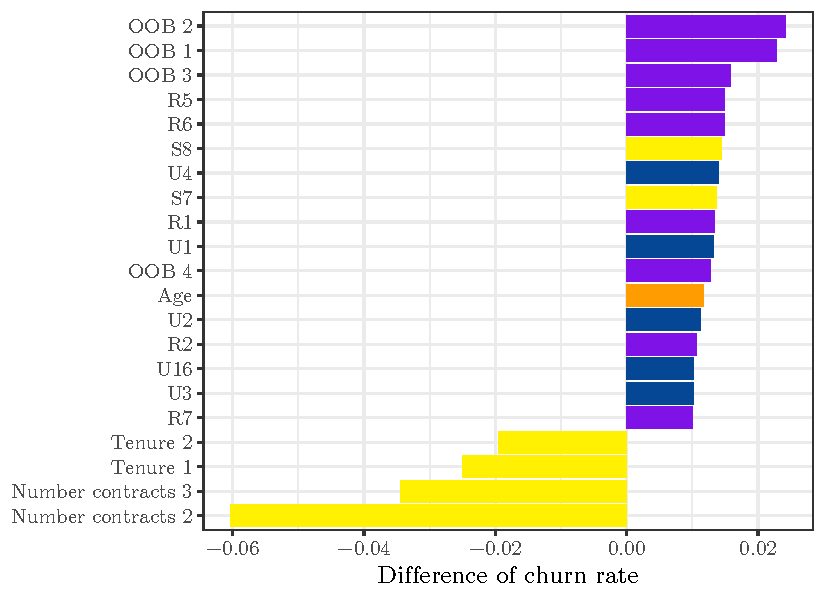
\includegraphics[width=0.9\linewidth]{figures/offset_1p.pdf}
    \caption{Difference in the predicted probability of churn when a standard
    deviation is added separately to each variable. Run on the SIM only dataset.
    Only variables inducing a difference having an absolute value greater than
    0.01 are shown.}
    \label{fig:offset_1p}
\end{figure}

\begin{figure}
    \centering
    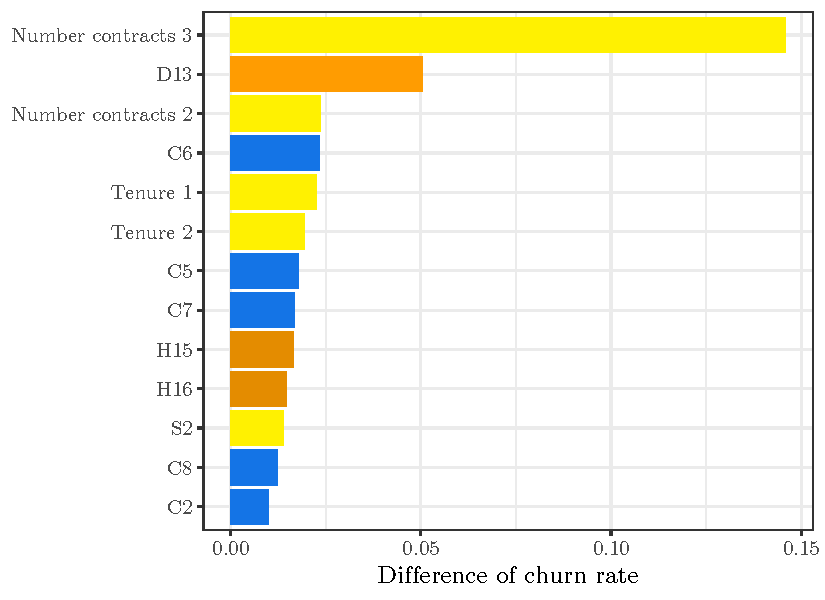
\includegraphics[width=0.9\linewidth]{figures/offset_1m.pdf}
    \caption{Difference in the predicted probability of churn when a standard
    deviation is subtracted separately from each variable. Run on the SIM only
    dataset. Only variables inducing a difference having an absolute value
    greater than 0.005 are shown.}
    \label{fig:offset_1m}
\end{figure}

\section{Comparison to the state of the art}

In this section, we compare our results to other studies in churn prediction. Of
the 20 articles in our bibliography related to churn prediction, 15 are
empirical studies either suggesting a new method or comparing existing methods.
7 of these 15 articles use precision, recall, accuracy, and F-measure as
evaluation measures. These evaluation measures are applicable when the output of
the prediction model is a hard label, such as for a support vector machine or a
decision tree. However, our experiment uses an ensemble model composed of random
forests and the predictions take the form of a score between 0 and 1. This
implies that a decision threshold has to be chosen when classifying customers as
churners or non-churners. The precision, recall, F-measure and accuracy are thus
functions of this threshold, and this does not allow a direct comparison with
these 7 empirical studies. We are left with 8 other studies which use either the
lift at different thresholds (most often 10\%, also named top decile lift), the
expected maximum profit and the area under the ROC curve (AUROC). The results of
these studies are compiled in table \ref{tab:comparison_sota}, along with our
results in the last row.

\begin{table}
    \centering
    \begin{tabular}{llrrr}
        \toprule
        Paper & Best method & AUROC & Lift 10\% & Lift 5\%\\
        \midrule
        \citeauthor*{coussement2017comparative}, \citeyear{coussement2017comparative}
        & Logistic regression & 0.63 & 2.19 & ---  \\
        \citeauthor*{decaigny2018new}, \citeyear{decaigny2018new}
        & Logit Leaf model & 0.87 & 5.34 & ---  \\
        \citeauthor*{oskarsdottir2018time}, \citeyear{oskarsdottir2018time}
        & Similarity forests & 0.87 & 6.05 & ---  \\
        \citeauthor*{zhu2017empirical}, \citeyear{zhu2017empirical}
        & C4.5 with UnderBagging & 0.80 & 4.54 & ---  \\
        \citeauthor*{mitrovic2018operational}, \citeyear{mitrovic2018operational}
        & Random forest & 0.74 & 2.35 & ---  \\
        \citeauthor*{idris2014ensemble}, \citeyear{idris2014ensemble}
        & Ensemble with mRMR & 0.75 & ---  & ---  \\
        \citeauthor*{oskarsdottir2017social}, \citeyear{oskarsdottir2017social}
        & Logistic Regression & 0.89 & ---  & 6.16 \\
        \citeauthor*{verbeke2014social}, \citeyear{verbeke2014social}
        & Relational classifier & ---  & 3.11 & 3.92 \\
        \addlinespace
        Our results & Easy Ensemble & 0.73 & 3.41 & 4.68 \\
        \bottomrule
    \end{tabular}
    \caption{Comparison of our results to other studies in churn prediction.}
    \label{tab:comparison_sota}
\end{table}

We consider our results on the SIM only test set, taking the results of one of
the best performing configurations (no variable selection, no difference or ratio
variables). It is important to notice that the studies mentioned in table
\ref{tab:comparison_sota} obviously do not provide a unique numerical result. In
each of these studies, we considered, whenever possible, the results pertaining
to a dataset similar to ours in terms of churn rate and type of contracts. Also,
when multiple methods are compared in a study, we retained the evaluation
measure of the method performing best. The name of the method retained in each
study is given in the second column of the table.

In terms of area under the ROC curve, we achieve results similar to 2 studies,
both using random forests (the ensemble proposed by \textcite{idris2014ensemble}
contains a random forest, a KNN, and a rotation forest). Also, we perform better
than the logistic regression proposed by \textcite{coussement2017comparative},
but the 4 remaining papers outperform our model by a clear margin. In terms of
lift, we outperform the logistic regression in the first row, the random forest
used in \textcite{mitrovic2018operational} and the combined relational
classifier proposed by \textcite{verbeke2014social}. All other studies yield a
superior lift, both at 5\% and 10\% threshold.

\section{Conclusion}

We summarize here the main findings of our experiments on churn prediction. All
those conclusions are inevitably strongly related to the limited dataset we
considered. We expect that further validation could help in better supporting
such conclusions. Also, the variable selection performed in these experiments
gives a useful, restricted scope for the causal analysis in the next chapter by
discarding irrelevant variables.

\begin{itemize}
    \item Feature selection does not reduce performance if at least 30 of the
    most important variables are selected.
    \item Adding difference and ratio variables reduces the performance if no
    feature selection is conducted beforehand.
    \item Due to a lucky domain shift, the trained models actually perform
    better on the test set than on the validation set.
    \item Churn is slightly easier to predict in the loyalty dataset, due to
    the importance of time-related variables.
    \item Important variables include non-exhaustively: the tenure, the
    province, the tariff plan, the number of calls, and the data usage.
    \item The tenure and the number of contracts are associated monotonically to
    the churn probability
    \item Variables related to the amount paid by the customer are associated to
    more churn when they are increased, but the opposite is not true.
\end{itemize}
